\documentclass[UTF8,a4paper,12pt]{ctexart}
\usepackage[a4paper,margin=2.5cm]{geometry}
\usepackage{amsmath,booktabs,longtable,array,graphicx,hyperref,enumitem,endnotes}
\usepackage{float}
\graphicspath{{graphics/}}
\hypersetup{colorlinks=true,linkcolor=black,urlcolor=blue}
\setlength{\parindent}{2em}
\setlength{\parskip}{0.35em}
\renewcommand{\contentsname}{目录}
\renewcommand{\figurename}{图}
\renewcommand{\tablename}{表}
\renewcommand{\notesname}{尾注}
\newcommand{\src}[1]{\endnote{#1}}

\title{石头科技扫地机产品在RCEP区域的国际市场开拓策划方案}
\author{小熊队\\
朱妍（国际经济与贸易（国际贸易/金融风险管理）25-4）\\
黄孝睿（经济学基地班25-0）\\
张语晗（金融学（北外联培25））}
\date{2026年9月}

\newpage

\begin{document}
\maketitle
\tableofcontents
\newpage

\section{产品概况}

\subsection{产品范围与企业基础}

本方案研究石头科技智能扫地机器人产品，企业主体为北京石头世纪科技股份有限公司，品牌名为Roborock。公司年报将智能扫地机器人列为核心主营产品，业务覆盖设计、研发、生产和销售；产品技术集中在环境感知、路径规划、清扫与拖地执行、基站自维护及移动端控制等环节。\src{北京石头世纪科技股份有限公司，《2025年年度报告》，第13--16页。}

扫地机器人不是单一的吸尘器替代品。消费者购买的是一套自动完成地面清洁的系统，产品价值由主机、基站、导航传感器、软件算法和售后服务共同构成。石头科技年报显示，公司正在推进机械臂扫地机、活水洗地等产品方向，并持续扩充不同价格带的产品矩阵。\src{石头科技，《2025年年度报告》，第14页。}

本研究把产品出口海关编码限定为中国海关申报码85098090.00。ITC工具实际采用HS6层级850980，对应“其他带自备电动机的机电家用器具”产品组。两者不是同一统计层级，因此本文的贸易规模、EPI和未实现潜力均称为“HS850980产品组数据”，用于评估扫地机相关产品的外部市场环境，不把产品组数值直接解释为Roborock品牌销售额。\src{中华人民共和国海关进出口税则，税号85098090；国际贸易中心（ITC），Trade Map与Export Potential Map，HS850980产品说明，访问日期2026年9月5日。}

\subsection{产品竞争要素}

扫地机在海外市场能否形成复购和口碑，取决于四个相互牵制的环节：第一，导航和避障能否适应不同住宅结构；第二，清扫、拖地及基站维护能否减少人工介入；第三，App、语音控制和售后服务能否降低使用门槛；第四，产品价格能否覆盖从尝鲜型消费者到高端家庭的多层需求。公司年报将智能操控、远程观察、路径规划和基站自维护列为技术演进的重要方向。\src{石头科技，《2025年年度报告》，第15--17页。}

对成熟市场，应突出产品可靠性、家庭场景适配和服务网络；对增长较快但规模较小的市场，应先用较少的SKU验证渠道、价格和售后成本，再决定是否扩大投入。

\subsection{世界生产与消费概况}

智能扫地机器人属于电子、机械、软件和家用电器交叉行业。中国具备较完整的家电供应链和电子制造基础，石头科技则把研发、品牌和产品定义置于供应链之上。石头科技年报指出，国内清洁电器渗透率仍有提升空间，海外市场已经成为企业增长的重要方向；公司同时通过品牌建设、全价格段覆盖和精细化渠道运营拓展海外用户。\src{石头科技，《2025年年度报告》，第10、15--16页。}

从消费侧看，扫地机器人更适合双职工家庭、养宠家庭、较大住宅和对清洁效率要求较高的消费者。不同市场的地面材质、门槛高度、住宅面积、网络环境和售后期待差异明显。产品进入RCEP市场后，主机配置可以保持相对统一，但说明书、App语言、插头规格、保修政策和渠道服务必须本地化。

\section{全球贸易概况}

\subsection{贸易数据口径}

本文采用ITC Trade Map、Market Access Map和Export Potential Map的数据。Trade Map覆盖2020--2025年，金额原始单位为千美元；EPM输出EPI潜力和基准出口额，金额为美元；Market Access Map记录目的国税则线、适用税率和非关税措施。\src{国际贸易中心（ITC），Trade Map、Export Potential Map与Market Access Map；产品HS850980，出口国为中国，目的市场为RCEP成员国，访问日期2026年9月5日。}

三套工具解决不同问题。Trade Map回答“市场是否足够大、增长是否持续、中国处在什么位置”；Export Potential Map把出口国供给、目标国需求和双边贸易便利度合并为EPI；Market Access Map核对税则线、适用税率和非关税措施。模型只在国家、产品、年份和单位对齐后连接三类数据，避免把贸易额、潜力值和关税写在同一列后直接比较。

\begin{table}[H]
\centering
\caption{ITC数据在本研究中的作用}
\label{tab:itcdata}
\small
\begin{tabular}{p{2.8cm}p{5.5cm}p{5.4cm}}
\toprule
工具 & 进入模型的字段 & 本文用途\\
\midrule
Trade Map & 2025年进口额、2020--2025年CAGR、中国供应份额与排名 & 衡量市场规模、增长及中国供应基础\\
Export Potential Map & EPI、基准出口额、未实现潜力及其比例 & 衡量未来可拓展空间\\
Market Access Map & 目的国税则线、实际适用税率、NTM记录 & 衡量市场准入成本并核对RCEP承诺\\
\bottomrule
\end{tabular}
\par\vspace{0.4em}
\begin{minipage}{0.92\textwidth}\small
资料来源：ITC三套工具的项目来源账本与字段说明，访问日期2026年9月5日。
\end{minipage}
\end{table}

\subsection{进口市场与中国供给}

表\ref{tab:top3}列出模型筛选出的前三个市场。日本2025年HS850980产品组进口额为531,328千美元，规模在候选市场中最大；韩国为307,301千美元，2020--2025年进口复合增长率为7.1221%；澳大利亚为203,135千美元，复合增长率为6.1031%。三国2025年中国供应商排名均为第1位，中国在三国进口中的份额分别为73.8088\%、84.1195\%和85.1193\%。\src{国际贸易中心（ITC），Trade Map，HS850980：日本、韩国和澳大利亚2020--2025年进口额及2025年按供应国进口数据，访问日期2026年9月5日。}

\begin{figure}[H]
\centering
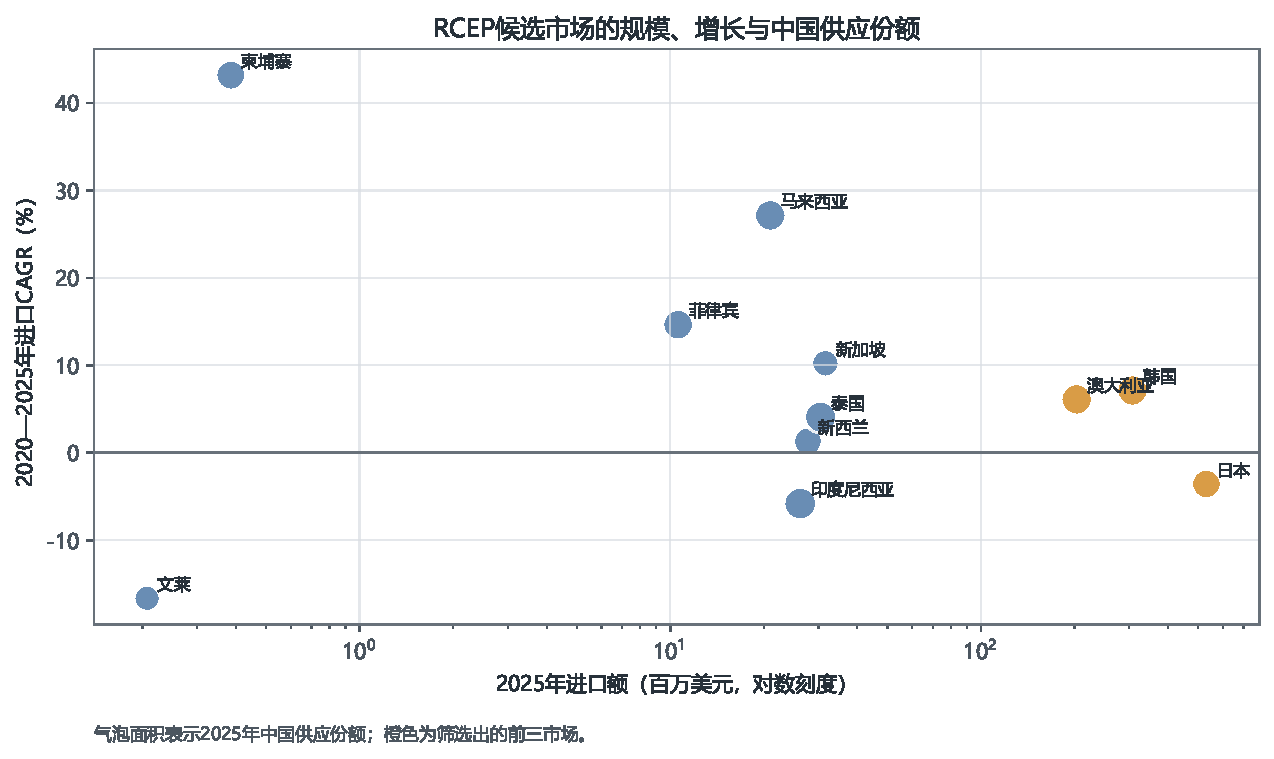
\includegraphics[width=0.92\textwidth]{market_size_growth.pdf}
\caption{RCEP候选市场的进口规模、增长率与中国供应份额}
\label{fig:sizegrowth}
\begin{minipage}{0.92\textwidth}\small
数据来源：ITC Trade Map，2020--2025年HS850980；仅绘制贸易字段完整的11个市场。横轴采用对数刻度，气泡面积表示2025年中国供应份额。
\end{minipage}
\end{figure}

\begin{table}[H]
\centering
\caption{前三市场的贸易与潜力指标}
\label{tab:top3}
\small
\begin{tabular}{lrrrrrr}
\toprule
市场 & 2025进口额 & 2020--25 CAGR & 中国份额 & EPI潜力 & 未实现潜力 & 适用税率\\
 & 千美元 & \% & \% & 美元 & 美元 & \%\\
\midrule
日本 & 531328 & -3.5686 & 73.8088 & 643300726 & 217232460 & 0\\
韩国 & 307301 & 7.1221 & 84.1195 & 459297135 & 160140835 & 0\\
澳大利亚 & 203135 & 6.1031 & 85.1193 & 209248488 & 63159688 & 0\\
\bottomrule
\end{tabular}
\par\vspace{0.4em}
\begin{minipage}{0.92\textwidth}\small
数据来源：ITC Trade Map、Export Potential Map和Market Access Map，2025年数据；本研究计算。
\end{minipage}
\end{table}

日本的优势来自大市场和较高的潜在空间，但其近期进口增速为负，说明市场成熟度较高，进入策略应避免单纯扩大投放。韩国市场规模次之且保持正增长，适合围绕高性能、智能化和本地售后建立稳定渠道。澳大利亚规模略小于韩国，但中国供应商地位稳固、进口保持增长，适合以高端机型和线上线下结合的方式推进。

图\ref{fig:sizegrowth}把规模与增长放在同一坐标中。柬埔寨和马来西亚的增速较高，但2025年进口额分别只有38.5万美元和2,097.5万美元；日本的进口额达到5.313亿美元，但五年CAGR为负。单独按增长率排序会偏向小基数市场，单独按规模排序又会忽略需求动能，因此市场筛选必须同时保留规模、增长和潜力指标。

\subsection{全球出口特点}

中国是该产品组的重要供给国。ITC Trade Map的中国对世界出口文件显示，中国电气机械及设备类出口规模大，HS850980的国别双边数据进一步显示，中国对候选市场已经形成较强供给基础。对本方案而言，这一基础意味着石头科技不必从零验证中国制造的可获得性，真正需要解决的是品牌差异化、渠道效率、合规和售后成本。

\begin{figure}[H]
\centering
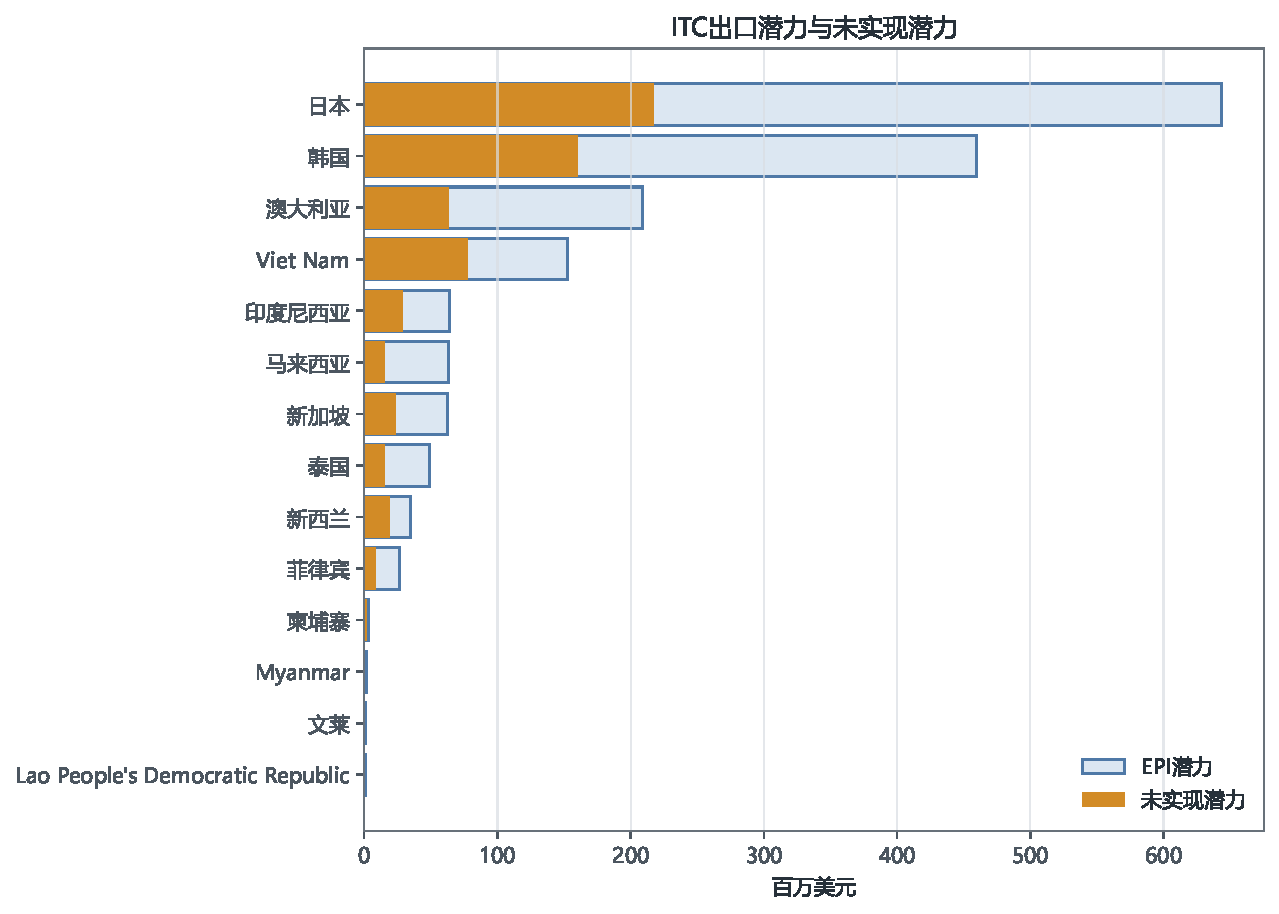
\includegraphics[width=0.92\textwidth]{epi_untapped.pdf}
\caption{中国向RCEP候选市场出口HS850980的EPI与未实现潜力}
\label{fig:epi}
\begin{minipage}{0.92\textwidth}\small
数据来源：ITC Export Potential Map，出口国为中国，产品组为HS850980，访问日期2026年9月5日。未实现潜力按各市场逐项计算，不用汇总差额替代。
\end{minipage}
\end{figure}

图\ref{fig:epi}显示，日本、韩国和澳大利亚的EPI绝对值明显高于多数东盟市场。越南的未实现潜力也较高，但Trade Map关键字段缺失，无法与其余市场按同一口径计算综合分数；因此越南保留在机会观察名单，没有进入本轮定量排名。

\section{中国出口业绩}

\subsection{出口表现}

按中国出口报告口径，2025年中国对日本、韩国和澳大利亚出口的HS850980产品组金额分别为309,129千美元、359,823千美元和183,021千美元。按进口国报告口径，三国自中国进口额分别为392,167千美元、258,500千美元和172,907千美元。进口与出口记录受FOB/CIF计价、运输时点和转口影响，本文用进口国口径计算目标市场份额，用中国出口口径观察中国的目的地结构。\src{国际贸易中心（ITC），Trade Map，HS850980：中国对日本、韩国和澳大利亚出口及三国自中国进口数据，2025年，访问日期2026年9月5日。}

\begin{table}[H]
\centering
\caption{前三市场的供应国竞争结构（2025年）}
\label{tab:competition}
\small
\begin{tabular}{lrrlrr}
\toprule
市场 & 中国份额 & 中国排名 & 第二供应国 & 第二供应国份额 & 份额差\\
 & \% & & & \% & 百分点\\
\midrule
日本 & 73.81 & 1 & 泰国 & 9.84 & 63.97\\
韩国 & 84.12 & 1 & 泰国 & 6.38 & 77.74\\
澳大利亚 & 85.12 & 1 & 德国 & 9.76 & 75.36\\
\bottomrule
\end{tabular}
\par\vspace{0.4em}
\begin{minipage}{0.92\textwidth}\small
数据来源：ITC Trade Map三国2025年按供应国进口派生表。
\end{minipage}
\end{table}

\begin{figure}[H]
\centering
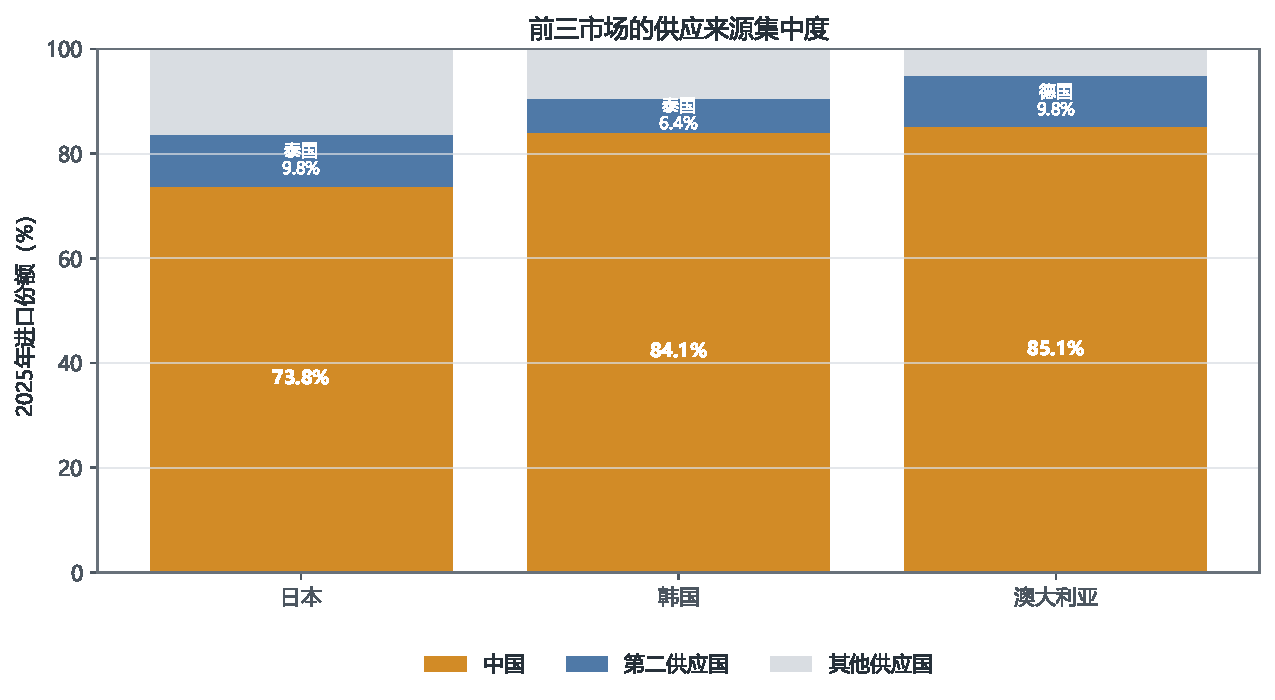
\includegraphics[width=0.84\textwidth]{supplier_concentration.pdf}
\caption{前三市场的供应来源集中度}
\label{fig:supplier}
\begin{minipage}{0.84\textwidth}\small
数据来源：ITC Trade Map三国2025年按供应国进口派生表。第二供应国在日本、韩国均为泰国，在澳大利亚为德国。
\end{minipage}
\end{figure}

图\ref{fig:supplier}显示，中国在三国均拥有超过七成的供应份额，竞争焦点已经从“能否进入”转向“谁能取得品牌溢价和渠道控制力”。石头科技在日韩需要同时面对区域内制造供给与本地渠道品牌，在澳大利亚还要与德国高价家电形象竞争。\src{国际贸易中心（ITC），Trade Map，HS850980：日本、韩国和澳大利亚2025年按供应国进口排名，访问日期2026年9月5日。}

\subsection{产品竞争力}

石头科技的优势在于技术密度和产品矩阵。公司年报记载的感知、决策、执行、基站自维护和移动端控制能力，能够支撑高端扫地机的产品溢价；但这些能力只有在当地形成稳定的安装、退换货和维修流程后，才会转化为持续竞争力。\src{石头科技，《2025年年度报告》，第13--17页。}

从中国供给份额看，前三市场中中国已经占据较高比例。进入策略因此不宜把“扩大中国来源”作为唯一目标，而应把目标改为：在中国供给优势之上，争取高端细分、改善品牌认知、降低售后成本，并建立可量化的渠道转化率和退货率监控。

\subsection{关税与产品归类}

Market Access Map返回的相关税则线中，澳大利亚、韩国和日本的当前适用税率记录为0\%。这为中国出口提供了成本条件，但零关税不等于无合规成本；不同国家仍可能存在电器安全、无线通信、能效、消费者保护、包装和售后义务。\src{国际贸易中心（ITC），Market Access Map，中国出口至日本、韩国和澳大利亚的HS850980相关税则线及实际适用税率，访问日期2026年9月5日。}

\section{市场筛选}

\subsection{ITC出口潜力框架}

ITC出口潜力指标把出口国供给能力、目标市场需求和双边贸易便利度结合起来。对出口国$i$、目标市场$j$和产品$k$，基本关系为

\begin{equation}
EPI_{ijk}=Supply_{ik}\times Ease_{ij}\times Demand_{ijk}.
\end{equation}

本研究直接使用Export Potential Map返回的官方EPI，不用自建回归值替代。未实现潜力在每个“中国—目的国—HS850980”组合上计算：

\begin{equation}
Untapped_{ijk}=\max\left(EPI_{ijk}-ActualExports_{ijk},0\right).
\end{equation}

这一处理使已经超过潜力基准的市场不会抵消其他市场的拓展空间。EPI提供的是供给、需求和双边条件共同形成的基准，适合用于跨市场比较；渠道费用、认证、售后和品牌份额仍需在市场进入方案中单独测算。\src{国际贸易中心（ITC），Export Potential Map方法说明及中国向RCEP成员国出口HS850980的EPI记录，访问日期2026年9月5日。}

\subsection{指标、变换与权重}

候选范围包括东盟十国、澳大利亚、新西兰、日本和韩国。老挝、缅甸和越南缺少完整的Trade Map进口规模、增长或中国份额，保留EPI结果但不进入综合排序；其余11个市场按统一口径建模。金额指标采用$\ln(1+x)$，避免日本、韩国等大市场的绝对规模完全压过中小市场；增长率、份额和潜力比例直接做极差标准化。正向指标的标准化公式为

\begin{equation}
z_{ij}=\frac{x_{ij}-\min(x_j)}{\max(x_j)-\min(x_j)}.
\end{equation}

\begin{table}[H]
\centering
\caption{市场吸引力模型的指标与战略权重}
\label{tab:weights}
\small
\begin{tabular}{p{3.2cm}p{3.4cm}p{3.2cm}r}
\toprule
指标 & 原始字段 & 变换 & 权重\\
\midrule
市场规模 & 2025年进口额 & $\ln(1+x)$后Min--Max & 0.30\\
市场增长 & 2020--2025年CAGR & Min--Max & 0.10\\
中国竞争位置 & 2025年中国供应份额 & Min--Max & 0.10\\
未实现潜力金额 & EPI减基准出口额 & $\ln(1+x)$后Min--Max & 0.30\\
未实现潜力比例 & 未实现潜力除以EPI & Min--Max & 0.20\\
\bottomrule
\end{tabular}
\par\vspace{0.4em}
\begin{minipage}{0.92\textwidth}\small
资料来源：ITC模型输入；权重由本研究按市场开拓目标设定。
\end{minipage}
\end{table}

权重围绕本方案的任务设置：进口规模和未实现潜力各占30\%，直接回答“市场多大”和“还能拓展多少”；潜力比例占20\%，防止只选择已经高度实现的大市场；增长和中国份额各占10\%，分别衡量需求动能和现有供应基础。该组权重用于战略情景，不称为专家AHP权重。为了观察权重选择是否改变结论，另行计算等权、熵权和5,000组随机扰动情景。\src{本研究根据ITC Trade Map与Export Potential Map数据构建标准化矩阵，并分别采用战略权重、等权和熵权进行TOPSIS排序；模型运行日期2026年9月6日。}

\subsection{TOPSIS排序过程}

标准化矩阵乘以权重得到$v_{ij}=w_jz_{ij}$。每个市场到正理想解和负理想解的距离分别为

\begin{equation}
D_i^+=\sqrt{\sum_j(v_{ij}-v_j^+)^2},\qquad
D_i^-=\sqrt{\sum_j(v_{ij}-v_j^-)^2},
\end{equation}

最终贴近度为

\begin{equation}
C_i=\frac{D_i^-}{D_i^++D_i^-}.
\end{equation}

$C_i$越高，市场在当前指标和权重下越接近理想组合。图\ref{fig:score}给出战略权重情景的结果。

\begin{figure}[H]
\centering
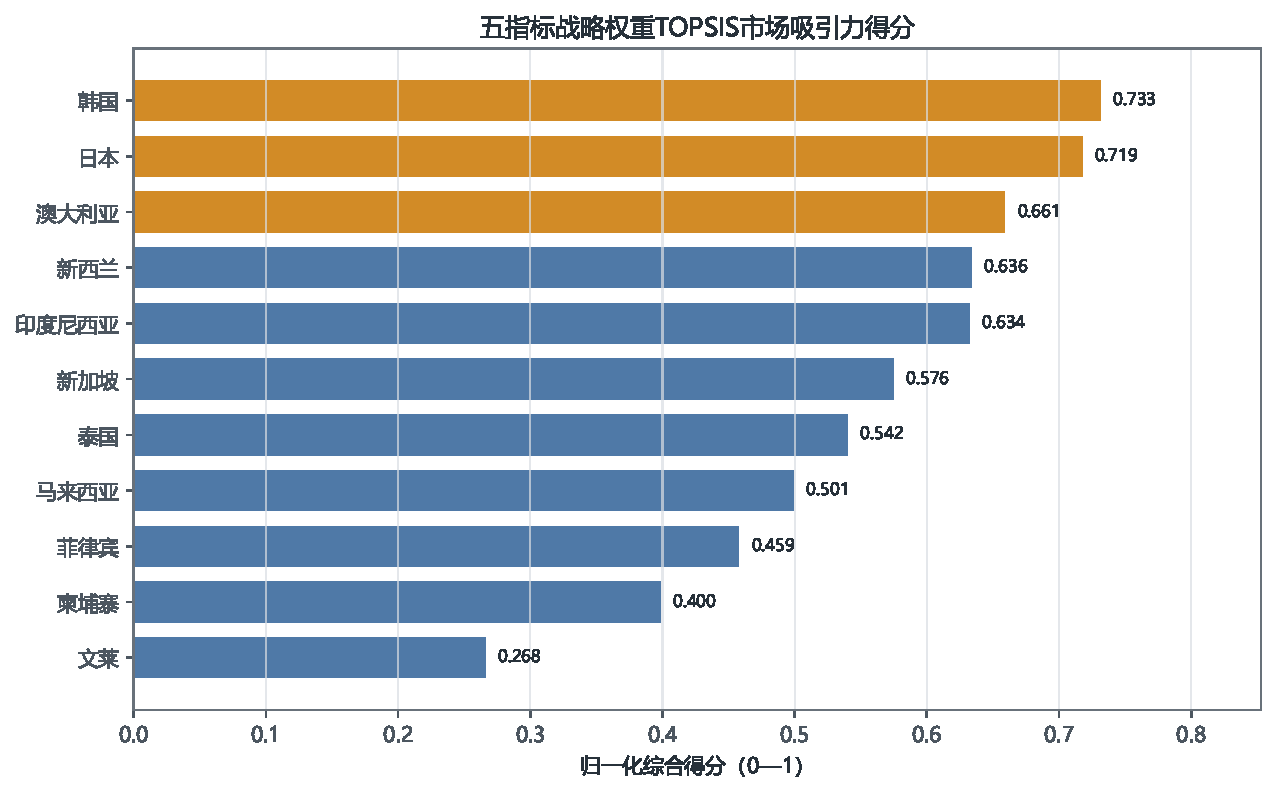
\includegraphics[width=0.90\textwidth]{market_score.pdf}
\caption{战略权重TOPSIS市场吸引力得分}
\label{fig:score}
\begin{minipage}{0.90\textwidth}\small
数据来源：ITC Trade Map、Export Potential Map和Market Access Map；本研究按表\ref{tab:weights}的指标与权重计算。橙色为前三市场。
\end{minipage}
\end{figure}

战略权重情景下，韩国得分0.733，日本0.719，澳大利亚0.661，构成第一梯队。新西兰和印度尼西亚分别为0.636和0.634，与澳大利亚接近，但绝对进口规模、未实现潜力金额或近期增速至少有一项明显偏弱。韩国的进口额和未实现潜力均居前列，五年增长为正；日本凭借候选市场中最大的进口额和未实现潜力保持第二；澳大利亚在规模、增长和中国份额之间最均衡。\src{本研究基于ITC五项市场指标计算的战略权重TOPSIS结果，模型运行日期2026年9月6日。}

\subsection{敏感性与选择结论}

等权、熵权和战略权重的排名存在差异。增长率和未实现比例权重提高时，柬埔寨、新西兰等市场会上升；规模和未实现潜力金额权重提高时，日本、韩国和澳大利亚更靠前。5,000组围绕战略权重的随机扰动中，韩国进入前三的比例为98.9\%，日本为90.6\%，澳大利亚为62.9\%；新西兰为30.6\%。韩国和日本的入选较稳定，澳大利亚与新西兰构成边界选择。澳大利亚最终入选，是因为其2025年进口规模约为新西兰的7.3倍，且中国供应份额和进口增速更高。

\begin{figure}[H]
\centering
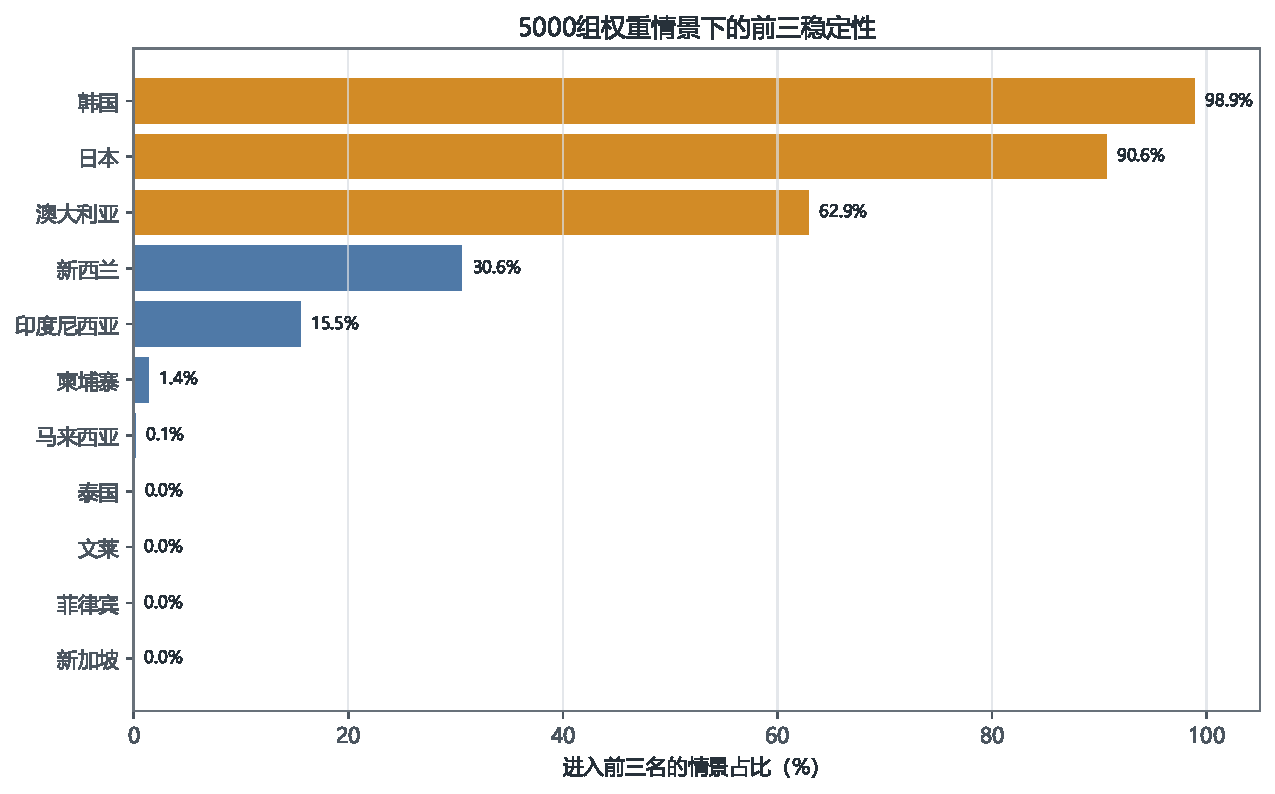
\includegraphics[width=0.90\textwidth]{ranking_sensitivity.pdf}
\caption{5,000组权重扰动情景下进入前三名的比例}
\label{fig:sensitivity}
\begin{minipage}{0.90\textwidth}\small
数据来源：ITC模型输入；本研究采用随机种子850980，权重由以战略权重为中心的Dirichlet分布生成。
\end{minipage}
\end{figure}

筛选结果由此确定为韩国、日本和澳大利亚。韩国承担近期增长与规模平衡，日本承担最大需求池，澳大利亚承担英语市场复制和渠道验证。三个市场的作用不同，资源配置也不应平均分配。

\section{目标市场特点}

\subsection{日本}

日本2025年进口额为5.313亿美元，ITC EPI为6.433亿美元，未实现潜力2.172亿美元，三项规模指标均居候选市场首位。五年进口CAGR为$-3.57\%$，说明可争取空间主要来自存量替换和品牌份额转移，而不是依赖市场自然扩张。日本市场应采用中高端主力机型与精简SKU组合，把地图准确性、低噪运行、边角清洁和耗材供应做成明确的体验指标。中国来源份额为73.81\%，石头科技需要用售后响应和产品稳定性与其他中国品牌拉开差异，而不是用低价证明中国制造能力。

\subsection{韩国}

韩国的进口额为3.073亿美元，五年CAGR为7.12\%，EPI为4.593亿美元，未实现潜力1.601亿美元。它没有日本的绝对规模，却同时具备正增长和较高潜力，因此在战略权重情景中排第一。韩国市场以高性能导航、基站自维护和智能控制为主卖点，上市顺序应当是售后合作方、备件仓、核心SKU，再扩大线上投放。中国来源份额已达84.12\%，消费者面对的是多家中国供应商，产品功能和售后承诺必须能在零售页面上直接比较。

\subsection{澳大利亚}

澳大利亚2025年进口额为2.031亿美元，五年CAGR为6.10\%，EPI为2.092亿美元，未实现潜力6,316万美元。进口规模约为新西兰的7.3倍，是敏感性分析中选择澳大利亚而不是新西兰的主要依据。产品测试应集中在地毯与硬质地面切换、毛发处理、较长运行时间和大户型覆盖。销售可由大型家电零售、品牌官网和平台电商共同承担，但三类渠道应使用统一的保修、耗材和退换货规则。

\subsection{季节性与备货节奏}

石头科技年报明确指出，海外Amazon等平台的Prime Day和Black Friday主要集中在第二季度和第四季度，这两个时段的销售额通常较高；促销高峰会同步放大采购、仓储、配送和售后压力。\src{北京石头世纪科技股份有限公司，《2025年年度报告》，“销售季节性风险”部分。}

三国可以共用一套备货节奏。第一季度完成新品认证、内容制作和渠道培训；第二季度围绕Prime Day形成第一轮销售峰值；第三季度根据退货率和维修数据调整库存；第四季度集中应对Black Friday和年末消费。日本和韩国的东亚仓可优先共享备件标准，澳大利亚库存则需提前考虑长距离补货。季节性管理的目标不是把销量压在促销日，而是避免促销订单转化为延迟交付和售后积压。

\subsection{价格定位与单位经济性}

公司年报显示，石头科技在海外推进全价格段覆盖。\src{北京石头世纪科技股份有限公司，《2025年年度报告》，“海外市场”和“全价格段布局”相关内容。} 对前三市场，价格体系可分为基础导航款、全能基站款和创新旗舰款，但每个市场先保留两到三个主力SKU。日本和韩国以全能基站款承担销量、旗舰款建立技术形象；澳大利亚增加适合大户型和地毯环境的配置。最终零售价应从目标贡献毛利倒推：

\begin{equation}
P=\frac{C_{FOB}+C_{freight}+C_{duty}+C_{channel}+C_{service}}{1-m},
\end{equation}

其中$m$为目标贡献毛利率，服务成本包括退换货、维修、备件和客服。三国当前适用关税记录均为0\%，价格差异将更多来自渠道扣点、物流和服务，而不是进口关税。

\section{前景分析}

\subsection{目标市场前景}

韩国提供较好的规模与增长组合，适合作为东亚市场的优先经营对象；日本拥有最大的潜在销售池，需要用产品体验争取存量替换；澳大利亚具有较清晰的中国供应基础和零关税条件，可检验品牌在英语市场的复制能力。三国分别承担增长、规模和复制任务，试销目标也应分开设定。

\subsection{人员、产品、许可与价格}

人员方面，需要本地市场经理、渠道经理、技术售后和客服人员，至少保证语言沟通、退换货和备件调度不依赖中国总部单点处理。产品方面，应保留核心导航和基站能力，同时适配当地插头、电压、语言和地面环境。许可方面，应在上市前完成当地电器安全、无线通信、能效和消费者保护要求的核对。价格方面，采用“主机价格加服务成本”的核算方法，避免以中国市场价格直接换算。

\subsection{RCEP规则的使用}

RCEP第2.4条要求成员方对原产货物按附件一承诺表实施关税减让；当实际最惠国税率更低时，进口商可以适用更低的最惠国税率。第2.6条进一步处理不同RCEP出口方税率存在差异时的“RCEP原产国”问题，第2.7条和第2.14条要求以协调制度进行商品归类并处理税表转版。对扫地机而言，这些条款把三个问题连在一起：先把中国申报码85098090.00映射到进口国税则线，再判断产品能否取得RCEP原产资格，最后比较RCEP税率与实际最惠国税率。\src{《区域全面经济伙伴关系协定》第2章“货物贸易”，第2.4、2.6、2.7和2.14条。}

\begin{table}[H]
\centering
\caption{前三市场HS8509.80相关税则承诺与当前准入结果}
\label{tab:rceptariff}
\small
\begin{tabular}{p{2.1cm}p{3.0cm}p{4.5cm}p{3.0cm}}
\toprule
市场 & 税则线 & RCEP承诺表 & ITC当前返回税率\\
\midrule
日本 & 850980.000 & Other appliances：Free & 0\%\\
韩国 & 8509.80.90.00 & 对中国表，基准8\%，第一年起0\% & 0\%\\
澳大利亚 & 8509.80.90 & 基准及所列年度均为0\% & 0\%\\
\bottomrule
\end{tabular}
\par\vspace{0.4em}
\begin{minipage}{0.92\textwidth}\small
资料来源：RCEP附件一日本、韩国对中国、澳大利亚关税承诺表；ITC Market Access Map，访问日期2026年9月5日。
\end{minipage}
\end{table}

三国的ITC当前适用税率均为0\%，承诺表与当前准入结果方向一致。日本承诺表直接列为Free；韩国对中国税表从第一年起降为0\%；澳大利亚8509.80.90在基准及各年度均为0\%。这使前三市场的竞争重点落在产品、渠道和服务上，而不是关税差异。\src{《区域全面经济伙伴关系协定》附件一关税承诺表：日本表第1133页、韩国对中国表第302页、澳大利亚表第102页；国际贸易中心（ITC），Market Access Map三国实际适用税率，访问日期2026年9月5日。}

取得优惠待遇的前提落在第3章。第3.2条规定原产货物的基本类型；HS2022产品特定原产地规则对8509.80给出“CTSH或RVC40”两条可选路径：非原产材料发生六位子目改变，或者区域价值成分达到40\%。\src{《区域全面经济伙伴关系协定》第3章第3.2条；《产品特定原产地规则（HS2022）》，税目8509.80，第118页。} 对石头科技而言，CTSH路径适合关键非原产零部件与整机归入不同六位子目的BOM；若部分核心部件与整机归类接近，则应转向RVC40并保存FOB价值、非原产材料价值和计算底稿。

第3.4条允许区域累积：来自其他RCEP成员方的原产材料用于中国生产时，可按规则视为中国生产中的原产材料。\src{《区域全面经济伙伴关系协定》第3章“原产地规则”，第3.4条“累积”。} 这对电机、传感器、芯片、电池或其他区域采购件具有直接意义。采购团队可以把“价格、性能、RCEP原产资格”同时纳入供应商选择；当CTSH路径不稳时，来自成员方的合格原产材料还能改善RVC40结果。

第3.6条排除仅包装、简单装配等微小加工，第3.7条允许在规定限度内处理未满足税则归类改变的少量非原产材料，第3.15条要求经第三方运输时保持海关监管并限制额外加工。第3.16至3.18条规定原产地证明方式和最低信息，第3.27条要求保存相关记录。\src{《区域全面经济伙伴关系协定》第3章第3.6、3.7、3.15、3.16--3.18和3.27条；《中华人民共和国海关〈区域全面经济伙伴关系协定〉项下进出口货物原产地管理办法》，海关总署令第255号。}

这些条款可转化为一套出口证据链：产品型号对应进口国税则线，BOM对应CTSH或RVC40计算，供应商声明支持区域累积，商业发票与原产地证明保持一致，提单和中转记录支持直接运输。证据链在首批出货前完成，后续每次BOM或供应商变化都触发原产资格复核。

RCEP第4章的预裁定、风险管理和货物放行条款可以降低通关不确定性；第6章对标准、技术法规和合格评定提出透明度与合作框架。扫地机仍要完成目的国的电器安全、电磁兼容、无线模块、电池和标签要求，但企业可以通过预裁定和提前提交完整技术文件减少归类与放行反复。\src{《区域全面经济伙伴关系协定》第4章“海关程序和贸易便利化”及第6章“标准、技术法规和合格评定程序”。}

\section{结论与行动安排}

本研究以中国海关编码85098090.00为产品输入，以ITC HS850980产品组完成市场筛选。战略权重TOPSIS的前三名为韩国、日本和澳大利亚。韩国在规模、正增长和未实现潜力之间最均衡；日本提供最大的进口规模和潜力金额；澳大利亚兼具正增长、高中国份额与英语市场复制价值。

\begin{table}[H]
\centering
\caption{市场进入的三阶段安排}
\label{tab:roadmap}
\small
\begin{tabular}{p{2.0cm}p{3.6cm}p{5.1cm}p{3.1cm}}
\toprule
阶段 & 时间与任务 & 主要交付 & 决策指标\\
\midrule
准备期 & 第1季度：归类、认证、渠道和售后签约 & 三国税则线确认、CTSH或RVC40底稿、核心SKU、备件清单 & 合规完成率、到岸成本、服务覆盖\\
试销期 & 第2季度至第3季度：Prime Day前后首轮销售 & 分渠道订单、退换货、维修和评价数据 & 转化率、退货率、维修周期、单台贡献毛利\\
扩张期 & 第4季度后：Black Friday及年度复盘 & 市场预算、库存和本地团队配置 & 获客成本、耗材复购、库存周转、前三稳定性\\
\bottomrule
\end{tabular}
\par\vspace{0.4em}
\begin{minipage}{0.92\textwidth}\small
资料来源：本研究依据ITC筛选结果、企业年报季节性信息与RCEP原产地规则设计。
\end{minipage}
\end{table}

资源配置不平均分配。韩国优先建立本地售后与旗舰产品认知，日本优先打磨中高端SKU和服务质量，澳大利亚优先验证大户型产品、零售渠道和长距离物流。试销数据进入下一轮模型，用品牌转化率、退货率、售后成本和单台贡献毛利替换目前缺失的企业层指标。这样，ITC的国家筛选结果才能落到石头科技自己的经营选择上。

\theendnotes

\end{document}
